\documentclass{standalone}
\usepackage{tikz}
\begin{document}
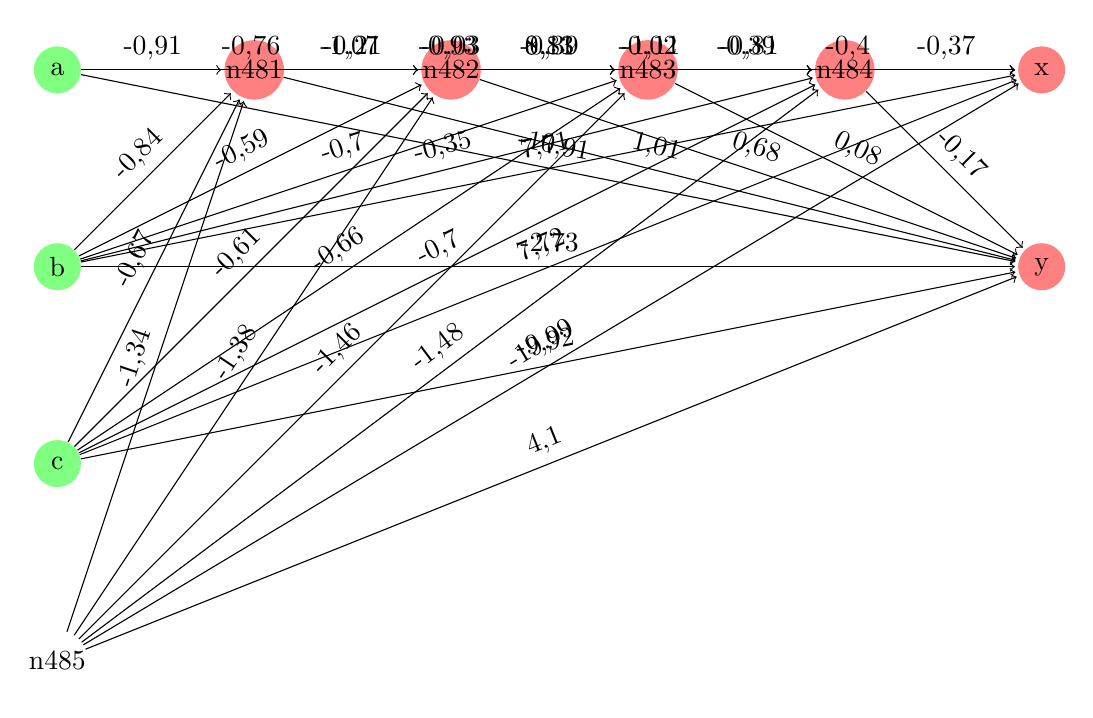
\begin{tikzpicture}[shorten >=1pt,->,draw=black!,node distance=2.5cm]
\tikzstyle{neuron}=[circle,fill=black!25,minimum size=17pt,inner sep=0pt]
\tikzstyle{constant}=[neuron, fill=white!50];
\tikzstyle{identity}=[neuron, fill=green!50];
\tikzstyle{sigmoid}=[neuron, fill=red!50];
\node [identity] (a) {a};
\node [identity,below of=a] (b) {b};
\node [identity,below of=b] (c) {c};
\node [constant,below of=c] (n485) {n485};
\node [sigmoid,right of=a] (n481) {n481};
\node [sigmoid,right of=n481] (n482) {n482};
\node [sigmoid,right of=n482] (n483) {n483};
\node [sigmoid,right of=n483] (n484) {n484};
\node [sigmoid,right of=n484] (x) {x};
\node [sigmoid,below of=x] (y) {y};
\path[every node/.style={sloped,anchor=south,auto=false}]
(c) edge node {7,72} (x)
(c) edge node {-0,67} (n481)
(c) edge node {-9,92} (y)
(c) edge node {-0,66} (n483)
(c) edge node {-0,61} (n482)
(c) edge node {-0,7} (n484)
(b) edge node {-2,73} (y)
(b) edge node {7,71} (x)
(b) edge node {-0,59} (n482)
(b) edge node {-0,84} (n481)
(b) edge node {-0,35} (n484)
(b) edge node {-0,7} (n483)
(a) edge node {8,81} (x)
(a) edge node {-0,93} (n484)
(a) edge node {-0,91} (n481)
(a) edge node {-10,91} (y)
(a) edge node {-1,07} (n483)
(a) edge node {-0,76} (n482)
(n482) edge node {-0,81} (x)
(n482) edge node {0,68} (y)
(n482) edge node {0,13} (n483)
(n482) edge node {-0,02} (n484)
(n481) edge node {1,01} (y)
(n481) edge node {-1,11} (x)
(n481) edge node {-0,39} (n484)
(n481) edge node {-0,21} (n482)
(n481) edge node {-0,03} (n483)
(n484) edge node {-0,17} (y)
(n484) edge node {-0,37} (x)
(n483) edge node {-0,4} (x)
(n483) edge node {0,08} (y)
(n483) edge node {-0,39} (n484)
(n485) edge node {4,1} (y)
(n485) edge node {-1,34} (n481)
(n485) edge node {-19,99} (x)
(n485) edge node {-1,48} (n484)
(n485) edge node {-1,38} (n482)
(n485) edge node {-1,46} (n483)
;\end{tikzpicture}
\end{document}